% !TeX encoding = UTF-8
\documentclass[11pt]{report}

% Paquetes y configuraciones adicionales
\usepackage{graphicx}
\usepackage[export]{adjustbox}
\usepackage{caption}
\usepackage{float}
\usepackage{titlesec}
\usepackage{geometry}
\usepackage[hidelinks]{hyperref}
\usepackage{titling}
\usepackage{titlesec}
\usepackage{parskip}
\usepackage{wasysym}
\usepackage{tikzsymbols}
\usepackage{fancyvrb}
\usepackage{xurl}
\usepackage{hyperref}

\usepackage{listings}
\usepackage{xcolor}
\usepackage{bashful}
\usepackage{bookmark}

\usepackage[spanish]{babel}

\newcommand{\subtitle}[1]{
  \posttitle{
    \par\end{center}
    \begin{center}\large#1\end{center}
    \vskip0.5em}
}

% Configura los márgenes
\geometry{
  left=2cm,   % Ajusta este valor al margen izquierdo deseado
  right=2cm,  % Ajusta este valor al margen derecho deseado
  top=3cm,
  bottom=3cm,
}

% Configuración de los títulos de las secciones
\titlespacing{\section}{0pt}{\parskip}{\parskip}
\titlespacing{\subsection}{0pt}{\parskip}{\parskip}
\titlespacing{\subsubsection}{0pt}{\parskip}{\parskip}

% Redefinir el formato de los capítulos y añadir un punto después del número
\makeatletter
\renewcommand{\@makechapterhead}[1]{%
  \vspace*{0\p@} % Ajusta este valor para el espaciado deseado antes del título del capítulo
  {\parindent \z@ \raggedright \normalfont
    \ifnum \c@secnumdepth >\m@ne
        \huge\bfseries \thechapter.\ % Añade un punto después del número
    \fi
    \interlinepenalty\@M
    #1\par\nobreak
    \vspace{10pt} % Ajusta este valor para el espacio deseado después del título del capítulo
  }}
\makeatother

% Configura para que cada \chapter no comience en una pagina nueva
\makeatletter
\renewcommand\chapter{\@startsection{chapter}{0}{\z@}%
    {-3.5ex \@plus -1ex \@minus -.2ex}%
    {2.3ex \@plus.2ex}%
    {\normalfont\Large\bfseries}}
\makeatother

% Configurar los colores para el código
\definecolor{codegreen}{rgb}{0,0.6,0}
\definecolor{codegray}{rgb}{0.5,0.5,0.5}
\definecolor{codepurple}{rgb}{0.58,0,0.82}
\definecolor{backcolour}{rgb}{0.95,0.95,0.92}

% Configurar el estilo para el código
\lstdefinestyle{mystyle}{
  backgroundcolor=\color{backcolour},   
  commentstyle=\color{codegreen},
  keywordstyle=\color{magenta},
  numberstyle=\tiny\color{codegray},
  stringstyle=\color{codepurple},
  basicstyle=\ttfamily\footnotesize,
  breakatwhitespace=false,         
  breaklines=true,                 
  captionpos=b,                    
  keepspaces=true,                 
  numbers=left,                    
  numbersep=11pt,                  
  showspaces=false,                
  showstringspaces=false,
  showtabs=false,                  
  tabsize=2
}

%==============================================================================
% Cosas para la documentación LateX
% % Sangría
% \setlength{\parindent}{1em}Texto

% % Quitar sangría
% \noindent

% % Punto
% \CIRCLE \ \ \textbf{Texto} \emph{algo}
% \begin{itemize}
%   \item \textbf{Negrita:} Texto
%   \item \textbf{Negrita:} Texto
% \end{itemize}

% % Introducir código
% \begin{center}
%   \begin{BVerbatim}
%     ... Código
%   \end{BVerbatim}
% \end{center}

% Poner una imagen
% \begin{figure}[H]
%   \centering
%   \includegraphics[scale=0.55]{img/}
%   \caption{Exportación de la base de datos en formato sql}
%   \label{fig:exportación de la base de datos en formato sql}
% \end{figure}

% Poner dos imágenes
% \begin{figure}[H]
%   \begin{subfigure}{0.5\textwidth}
%     \centering
%     \includegraphics[scale=0.45]{img/}
%     \caption{Texto imagen 1}
%   \end{subfigure}%
%   \begin{subfigure}{0.5\textwidth}
%     \centering
%     \includegraphics[scale=0.45]{img/}
%     \caption{Texto imagen 2}
%   \end{subfigure}
%   \caption{Texto general}
% \end{figure}

% % Poner una tabla
% \begin{table}[H]
%   \centering
%   \begin{tabular}{|c|c|c|c|}
%     \hline
%     \textbf{Campo 1} & \textbf{Campo 2} & \textbf{Campo 3} & \textbf{Campo 4} \\ \hline
%     Texto & Texto & Texto & Texto \\ \hline
%     Texto & Texto & Texto & Texto \\ \hline
%     Texto & Texto & Texto & Texto \\ \hline
%     Texto & Texto & Texto & Texto \\ \hline
%   \end{tabular}
%   \caption{Nombre de la tabla}
%   \label{tab:nombre de la tabla}
% \end{table}

% % Poner codigo de un lenguaje a partir de un archivo
% \lstset{style=mystyle}
% The next code will be directly imported from a file
% \lstinputlisting[language=Python]{code.py}

%==============================================================================

\begin{document}

% Portada del informe
\title{Práctica 10. Gestión de contraseñas}
\subtitle{Seguridad de Sistemas Informáticos}
\author{Cheuk Kelly Ng Pante (alu0101364544@ull.edu.es)}
\date{\today}

\maketitle

\pagestyle{empty} % Desactiva la numeración de página para el índice

% Índice
\tableofcontents

% Nueva página
\cleardoublepage

\pagestyle{plain} % Vuelve a activar la numeración de página
\setcounter{page}{1} % Reinicia el contador de página a 1

% Secciones del informe
% Capitulo 1
\chapter{Instalación de paquetes}
\begin{itemize}
  \item \textbf{pwgen.} Generador de contraseñas fuertes:
  \begin{BVerbatim}
sudo apt-get install pwgen
  \end{BVerbatim}
  \begin{figure}[H]
    \centering
    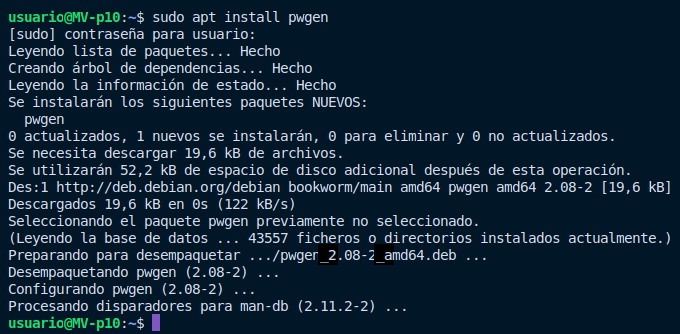
\includegraphics[scale=0.45]{img/pwgen_instalation.png}
    \caption{Instalación de pwgen}
    \label{fig:instalación de pwgen}    
  \end{figure}

  \item \textbf{makepasswd.} Generador de contraseñas aleatorias seguras y fiables:
  \begin{BVerbatim}
sudo apt-get install makepasswd
  \end{BVerbatim}
  \begin{figure}[H]
    \centering
    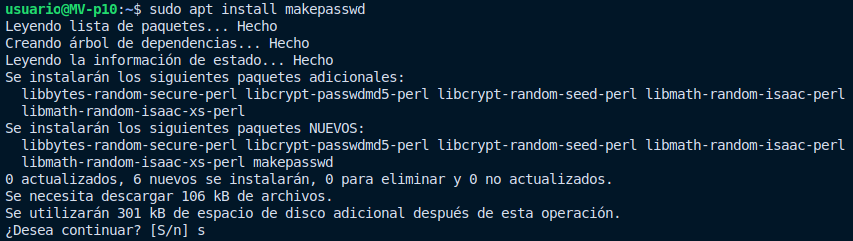
\includegraphics[scale=0.4]{img/makepasswd_instalation.png}
    \caption{Instalación de makepasswd}
    \label{fig:instalación de makepasswd}
  \end{figure}

  \item \textbf{apg.} Generador automático de contraseñas:
  \begin{BVerbatim}
sudo apt-get install apg
  \end{BVerbatim}
  \begin{figure}[H]
    \centering
    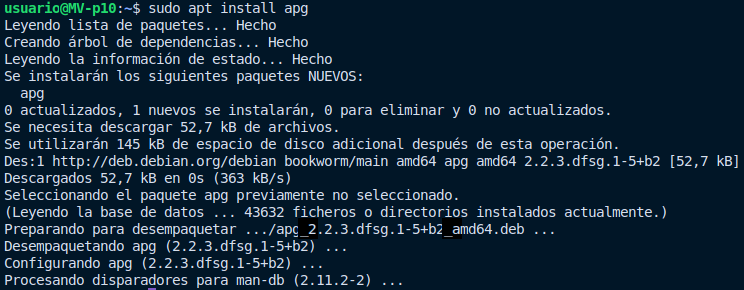
\includegraphics[scale=0.4]{img/apg_instalation.png}
    \caption{Instalación de apg}
    \label{fig:instalación de apg}
  \end{figure}

  % % Nueva página
  % \cleardoublepage

  \item \textbf{john (John The Ripper).} Crackeador de contraseñas:
  \begin{BVerbatim}
sudo apt-get install john
  \end{BVerbatim}
  \begin{figure}[H]
    \centering
    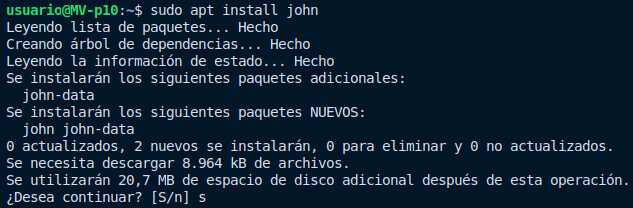
\includegraphics[scale=0.45]{img/john_instalation.png}
    \caption{Instalación de john}
    \label{fig:instalación de john}
  \end{figure}


\end{itemize}

% Capitulo 2
\chapter{Generar un fichero de contraseñas con hashes MD5}
Para generar un fichero de contraseñas con hashes MD5, se utilizará la herramienta \emph{makepasswd} pero 
como se está usando una máquina virtual del IAAS de la ULL y estas máquinas tienen
baja entropía en el generador de números aleatorios, hay que instalar y configurar \emph{haveged} para
resolverlo. Para ello, se ejecuta el siguiente comando:
\begin{BVerbatim}
sudo apt-get install haveged
\end{BVerbatim}
y configuramos el fichero \emph{/etc/default/haveged} asegurando que la variable \emph{DAEMON\_ARGS} 
contenga lo siguiente:
\begin{BVerbatim}
DAEMON_ARGS="-w 1024"
\end{BVerbatim}
. Una vez hecho esto, hay que estar seguro de que el servicio \emph{haveged} se está ejecutando:
\begin{BVerbatim}
update-rc.d haveged defaults
\end{BVerbatim}

Ahora, se puede generar el fichero de contraseñas con hashes MD5 con el siguiente comando:
\lstset{style=mystyle}
\lstinputlisting[language=bash]{gen_pass_md5.sh}

\begin{figure}[H]
  \centering
  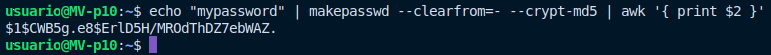
\includegraphics[scale=0.8]{img/gen_pass_md5.png}
  \caption{Generación de contraseñas con hashes MD5}
  \label{fig:generación de contraseñas con hashes MD5}
\end{figure}

% Nueva página
\cleardoublepage

\chapter{Creacion de usuarios con contraseñas generadas por \emph{pwgen}}
Para crear usuarios con contraseñas generadas por \emph{pwgen}, se ha creado un script que genera
cinco usuarios con contraseñas de menor a mayor fortaleza. El script es el siguiente:
\lstset{style=mystyle}
\lstinputlisting[language=Bash]{create_users.sh}

Al ejecutar el script, se crean los usuarios con las contraseñas generadas por \emph{pwgen}:
\begin{figure}[H]
  \centering
  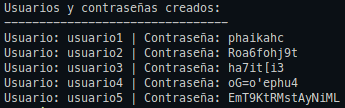
\includegraphics[scale=0.8]{img/users_creation.png}
  \caption{Creación de usuarios con contraseñas generadas por \emph{pwgen}}
  \label{fig:creación de usuarios con contraseñas generadas por pwgen}
\end{figure}

Una vez creado los usuarios, vamos a proceder a hacer un paso básico que es el "desombreado" que es 
un proceso en el que se combian el fichero \emph{/etc/passwd} y \emph{/etc/shadow} para que el hash de
la contraseña se encuentre en el fichero \emph{/etc/passwd} y no en el fichero \emph{/etc/shadow}. Para
ello, se ejecuta el siguiente comando:
\lstset{style=mystyle}
\lstinputlisting[language=Bash]{unshadow.sh}

Ahora el fichero \emph{unshadowed.txt} tendrá el siguiente contenido:
\begin{figure}[H]
  \centering
  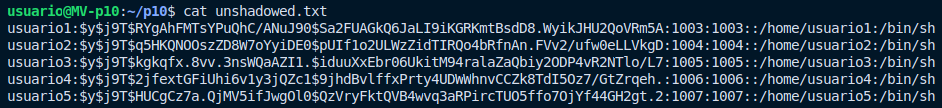
\includegraphics[scale=0.52]{img/unshadowed.png}
  \caption{Contenido del fichero \emph{unshadowed.txt}}
  \label{fig:contenido del fichero unshadow.txt}
\end{figure}

% Nueva página
\cleardoublepage

\chapter{Crackear las contraseñas con la herramienta \emph{John the Ripper}}


% Nueva página
\cleardoublepage

\chapter{Bibliografía} % En formato APA
\begin{enumerate}
\item LaMendola, S. (2013). How to Setup Additional Entropy for Cloud Servers Using Haveged. DigitalOcean. Recuperado de \url{https://www.digitalocean.com/community/tutorials/how-to-setup-additional-entropy-for-cloud-servers-using-haveged}
\item erev0s. (2020). Cracking /etc/shadow with John. Recuperado de \url{https://erev0s.com/blog/cracking-etcshadow-john/}  
\end{enumerate}

\end{document}